\documentclass{standalone}
\usepackage{tikz,color}

\definecolor{darkgreen}{RGB}{0,150,0}
\definecolor{darkred}{RGB}{200,0,0}

\begin{document}
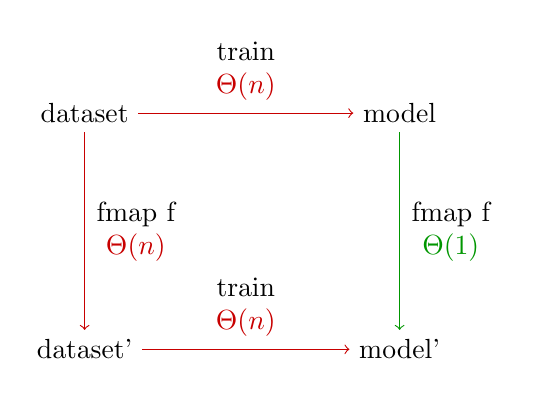
\begin{tikzpicture}
\node (xs)  {dataset};
\node[below of=xs,node distance=3cm] (xs2) {dataset'};
\node[right of=xs,node distance=4cm] (m1) {model};
\node[below of=m1,node distance=3cm] (m2) {model'};

\draw[->,draw=darkred] (xs) to node[right] {
    \hspace{-0.3cm}
    \begin{tabular}{c}
    fmap f\\
    \textcolor{darkred}{$\Theta(n)$}
    \end{tabular}
    }  (xs2);
\draw[->,draw=darkgreen] (m1) to node[right] {
    \hspace{-0.3cm}
    \begin{tabular}{c}
    fmap f\\
    \textcolor{darkgreen}{$\Theta(1)$}
    \end{tabular}
    }  (m2);
\draw[->,draw=darkred] (xs) to node[above] {
    \begin{tabular}{c}
    train\\
    \textcolor{darkred}{$\Theta(n)$}
    \end{tabular}
    }  (m1);
\draw[->,draw=darkred] (xs2) to node[above] {
    \begin{tabular}{c}
    train\\
    \textcolor{darkred}{$\Theta(n)$}
    \end{tabular}
    }  (m2);
\end{tikzpicture}
\end{document}
